\documentclass[12pt]{article}
\usepackage{amsmath}
\usepackage{graphicx}
\usepackage{caption}
\usepackage{float}
\usepackage[utf8]{inputenc}
\usepackage[T1]{fontenc}
\usepackage{geometry}
\usepackage{setspace}
\usepackage{parskip}
\usepackage[bottom]{footmisc}
\usepackage[table]{xcolor}
\usepackage{tikz}
\usetikzlibrary{positioning,fit,calc,arrows.meta,shapes.geometric}
\usepackage[english]{babel}
\usepackage{tabularx}
\usepackage{array}
\usepackage{colortbl}
\usepackage{enumitem}
\usepackage[hidelinks]{hyperref}
\usepackage{indentfirst}
\geometry{a4paper, margin=1in}

\usepackage{listings}
\lstset{
    basicstyle=\ttfamily\footnotesize,
    breaklines=true,
    frame=single,
    backgroundcolor=\color{gray!10},
    keywordstyle=\color{blue!70!black},
    commentstyle=\color{green!50!black},
    stringstyle=\color{red!60!black},
    showstringspaces=false,
    language=C
}

\definecolor{stellantis}{RGB}{26,58,92}
\definecolor{sectionblue}{RGB}{44,95,138}
\definecolor{ddbrownlight}{RGB}{255,243,230}
\definecolor{ddbrown}{RGB}{180,100,30}

\usepackage[most]{tcolorbox}
\tcbuselibrary{breakable}

\renewcommand{\arraystretch}{1.3}

\begin{document}

\begin{center}
{\LARGE\bfseries\color{stellantis} Task C --- Execution (PID Brake + Alert)}\\[6pt]
{\large Design Document}\\[10pt]
{\normalsize J\'essica Roberta de Souza Santos}\\
{\small April 2026}
\end{center}

\vspace{0.5cm}

% ======================================================================
\section{Overview}

This document describes the design choices, data flow, and requirements traceability for the Execution module of the AEB system. The module comprises two source files: \texttt{aeb\_pid.c} (PI brake controller) and \texttt{aeb\_alert.c} (alert mapping and driver override detection).

The module implements \textbf{FR-BRK-001 through FR-BRK-007} (braking control) and \textbf{FR-ALR-001 through FR-ALR-004} (driver alerts), plus \textbf{FR-DEC-006} and \textbf{FR-DEC-007} (driver override conditions) from SRS v2.0. The implementation is derived from three Simulink charts: \texttt{chart\_96} (PID\_Logic), \texttt{chart\_79} (Alert\_Map), and \texttt{chart\_88} (Override\_Det).

% ======================================================================
\section{Architecture and Data Flow}

\subsection{Position in the System}

The Execution module sits in the \textbf{Controller thread} (priority~2, 10\,ms cycle) and transforms FSM decisions into physical actuator commands:

\begin{figure}[H]
\centering
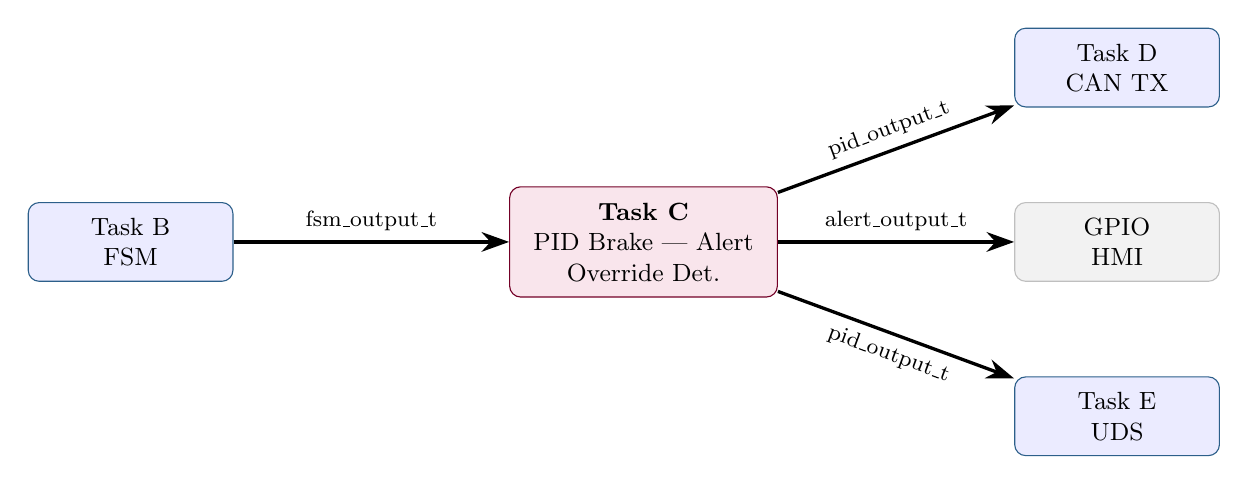
\begin{tikzpicture}[
    node distance=1.2cm and 2.8cm,
    mod/.style={rectangle, draw, rounded corners=4pt, minimum width=2.6cm, minimum height=1.0cm, font=\small, align=center},
    exec/.style={mod, fill=purple!10, draw=purple!60!black, minimum width=3.4cm, minimum height=1.4cm},
    ext/.style={mod, fill=gray!10, draw=gray!50},
    int/.style={mod, fill=blue!8, draw=sectionblue},
    arr/.style={-{Stealth[length=3.5mm, width=2.5mm]}, very thick},
    lbl/.style={font=\footnotesize}
]
    \node[int] (fsm) {Task B\\FSM};
    \node[exec, right=3.5cm of fsm] (exec) {\textbf{Task C}\\PID Brake | Alert\\Override Det.};
    \node[int, above right=1.0cm and 3.0cm of exec] (can) {Task D\\CAN TX};
    \node[ext, right=3.0cm of exec] (gpio) {GPIO\\HMI};
    \node[int, below right=1.0cm and 3.0cm of exec] (uds) {Task E\\UDS};

    \draw[arr] (fsm) -- (exec) node[lbl, above, midway] {fsm\_output\_t};
    \draw[arr] (exec) -- (can) node[lbl, above, midway, sloped] {pid\_output\_t};
    \draw[arr] (exec) -- (gpio) node[lbl, above, midway] {alert\_output\_t};
    \draw[arr] (exec) -- (uds) node[lbl, below, midway, sloped] {pid\_output\_t};
\end{tikzpicture}
\caption{Execution module data flow within the AEB system.}
\end{figure}

\subsection{Simulink Model Reference}

The implementation maps directly to three Simulink charts from \texttt{AEB\_Integration.slx}:

\begin{table}[H]
\centering
\caption{Simulink chart to C function mapping.}
\footnotesize
\begin{tabularx}{\textwidth}{|>{\raggedright\arraybackslash}p{2.5cm}
                              |>{\raggedright\arraybackslash}p{2.5cm}
                              |>{\raggedright\arraybackslash}X|}
\hline
\rowcolor{sectionblue}
\textcolor{white}{\textbf{Simulink Chart}} &
\textcolor{white}{\textbf{C Function}} &
\textcolor{white}{\textbf{Description}} \\ \hline

chart\_96 (PID\_Logic) & \texttt{pid\_brake\_step()} & PI controller with anti-windup and jerk limiting \\ \hline
chart\_79 (Alert\_Map) & \texttt{alert\_map()} & FSM state to alert type and buzzer pattern \\ \hline
chart\_88 (Override\_Det) & \texttt{override\_detect()} & Brake pedal and steering override detection \\ \hline

\end{tabularx}
\end{table}

% ======================================================================
\section{Design Choices}

\subsection{PI Controller with Anti-Windup}

The brake controller uses a PI control law with proportional gain $K_p = 10.0$ and integral gain $K_i = 0.05$:

\begin{equation}
e(k) = a_{\text{target}} - a_{\text{ego}}, \qquad
I(k) = I(k{-}1) + K_i \cdot e(k) \cdot \Delta t, \qquad
u(k) = K_p \cdot e(k) + I(k)
\end{equation}

The integral term is clamped to $[0,\,50\%]$ (anti-windup). The lower bound of zero prevents negative integral accumulation, since the AEB system only brakes --- it never commands acceleration.

\begin{tcolorbox}[colback=ddbrownlight, colframe=ddbrown, title=\textbf{Design Decision: Integral clamp at zero}]
Unlike a general-purpose PID, the AEB PI only produces positive brake commands. Allowing negative integral would mean the controller ``wants to accelerate,'' which is the FSM's responsibility (state transition to STANDBY). Clamping at zero ensures clean reset behaviour.
\end{tcolorbox}

\subsection{Jerk Limiting}

Longitudinal jerk is limited to $|\dot{a}| \leq 10$\,m/s$^3$ (FR-BRK-004). This is converted to a maximum output change per cycle:

\begin{equation}
\Delta u_{\max} = J_{\max} \times \frac{100\%}{a_{\max}} \times \Delta t = 10 \times \frac{100}{6} \times 0.01 \approx 1.667\,\%/\text{cycle}
\end{equation}

This also satisfies FR-BRK-001 (no jumps $> 2$\,m/s$^2$ between cycles), since $1.667\%$ maps to approximately $1.0$\,m/s$^2$ per cycle.

\subsection{Controller State Reset}

The PI integrator and previous output are reset to zero when the FSM leaves braking states ($\texttt{fsm\_state} < \texttt{FSM\_BRAKE\_L1}$) or when \texttt{decel\_target} $\leq 0$. This prevents integrator carry-over when the system transitions through WARNING $\to$ STANDBY $\to$ BRAKE\_L1 again.

\subsection{Alert Mapping as Pure Combinational Logic}

The \texttt{alert\_map()} function is stateless --- a direct lookup from FSM state to alert outputs. The 800\,ms minimum warning time (FR-ALR-003) is enforced by the FSM module (Task~B), not by the alert module. This keeps the function simple and testable.

\subsection{Override Detection Scope}

The \texttt{override\_detect()} function reports the general case: brake pedal OR steering angle $> 5^{\circ}$. The POST\_BRAKE exception (FR-FSM-006: only accelerator triggers override) is handled by the FSM module, which ignores the override signal in that state. This maintains separation of concerns.

\begin{tcolorbox}[colback=ddbrownlight, colframe=ddbrown, title=\textbf{Design Decision: No HAL abstraction needed}]
Unlike Task~D (CAN), the Execution module has no hardware dependencies. Both \texttt{pid\_brake\_step()} and \texttt{alert\_map()} are pure functions that receive structs and produce structs. No stubs directory is needed for host testing.
\end{tcolorbox}

% ======================================================================
\section{Execution Flow}

\begin{figure}[H]
\centering
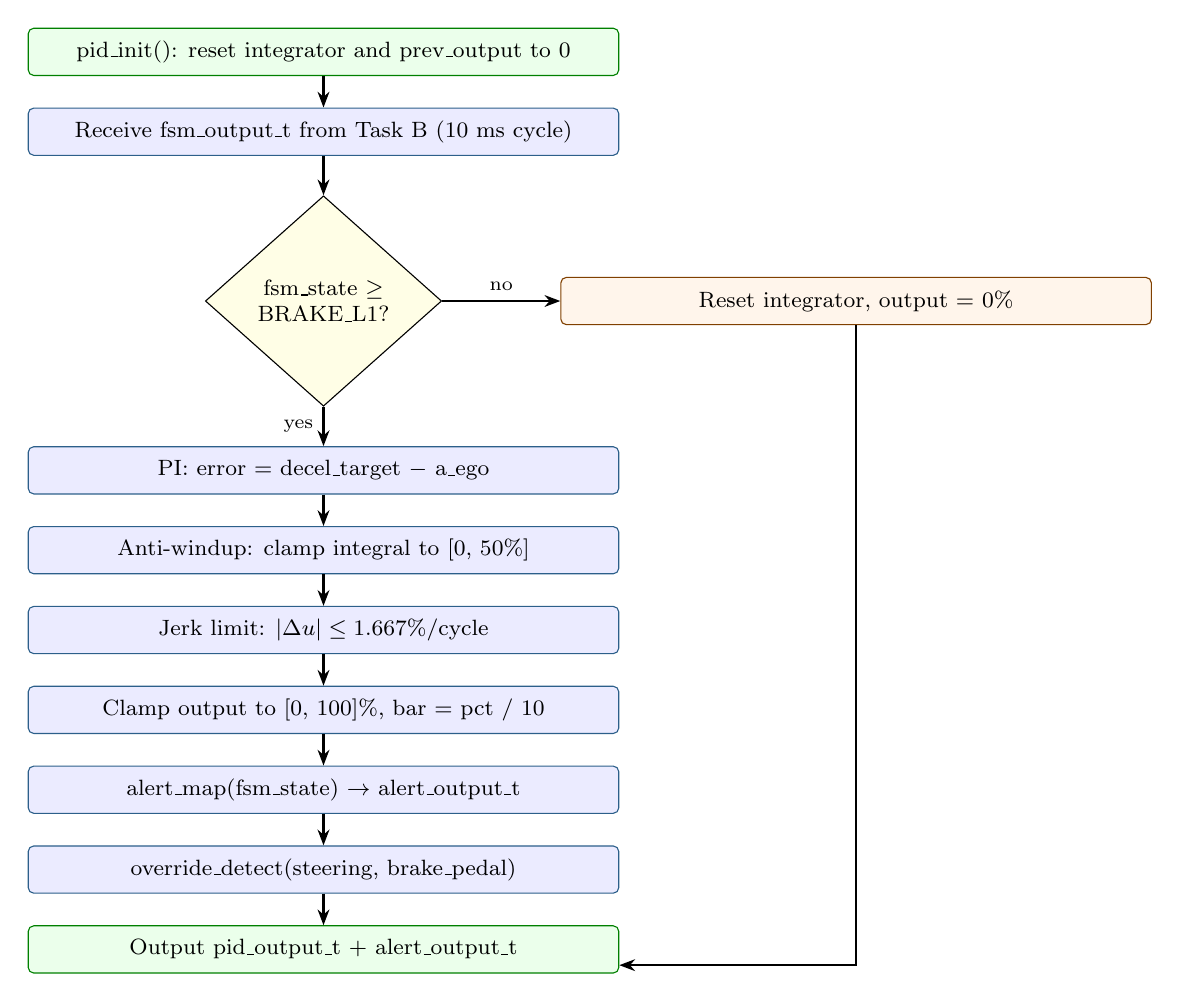
\begin{tikzpicture}[
    node distance=0.4cm,
    stp/.style={rectangle, draw, rounded corners=2pt, minimum width=7.5cm, minimum height=0.6cm, font=\footnotesize, align=center},
    s1/.style={stp, fill=green!8, draw=green!50!black},
    s2/.style={stp, fill=blue!8, draw=sectionblue},
    s3/.style={stp, fill=orange!8, draw=orange!50!black},
    dec/.style={diamond, draw, minimum width=3.0cm, minimum height=1.0cm, font=\footnotesize, align=center, fill=yellow!10},
    arr/.style={-{Stealth[length=2mm]}, thick}
]
    \node[s1] (init) {pid\_init(): reset integrator and prev\_output to 0};
    \node[s2, below=of init] (rcv) {Receive fsm\_output\_t from Task B (10 ms cycle)};
    \node[dec, below=0.5cm of rcv] (check) {fsm\_state $\geq$\\BRAKE\_L1?};
    \node[s3, right=1.5cm of check] (reset) {Reset integrator, output = 0\%};
    \node[s2, below=0.5cm of check] (pi) {PI: error = decel\_target $-$ a\_ego};
    \node[s2, below=of pi] (aw) {Anti-windup: clamp integral to [0, 50\%]};
    \node[s2, below=of aw] (jerk) {Jerk limit: $|\Delta u| \leq 1.667$\%/cycle};
    \node[s2, below=of jerk] (clamp) {Clamp output to [0, 100]\%, bar = pct / 10};
    \node[s2, below=of clamp] (alert) {alert\_map(fsm\_state) $\to$ alert\_output\_t};
    \node[s2, below=of alert] (ovr) {override\_detect(steering, brake\_pedal)};
    \node[s1, below=of ovr] (done) {Output pid\_output\_t + alert\_output\_t};

    \draw[arr] (init) -- (rcv);
    \draw[arr] (rcv) -- (check);
    \draw[arr] (check) -- node[font=\scriptsize, above] {no} (reset);
    \draw[arr] (check) -- node[font=\scriptsize, left] {yes} (pi);
    \draw[arr] (pi) -- (aw);
    \draw[arr] (aw) -- (jerk);
    \draw[arr] (jerk) -- (clamp);
    \draw[arr] (clamp) -- (alert);
    \draw[arr] (alert) -- (ovr);
    \draw[arr] (ovr) -- (done);
    \draw[arr] (reset.south) |- ([yshift=-2mm]done.east);
\end{tikzpicture}
\caption{Execution module flow per 10\,ms cycle.}
\end{figure}

% ======================================================================
\section{Requirements Traceability}

\begin{table}[H]
\centering
\caption{Traceability: SRS requirements $\to$ implementation.}
\scriptsize
\setlength{\tabcolsep}{3pt}
\begin{tabularx}{\textwidth}{|>{\raggedright\arraybackslash}p{1.5cm}
                              |>{\raggedright\arraybackslash}p{2.5cm}
                              |>{\raggedright\arraybackslash}p{3.0cm}
                              |>{\raggedright\arraybackslash}X|}
\hline
\rowcolor{sectionblue}
\textcolor{white}{\textbf{Req.}} &
\textcolor{white}{\textbf{Requirement}} &
\textcolor{white}{\textbf{Implementation}} &
\textcolor{white}{\textbf{Test}} \\ \hline

FR-BRK-001 & Progressive decel., no jumps $> 2$\,m/s$^2$ & Jerk limiter in pid\_brake\_step() & test\_pid\_no\_abrupt\_jumps \\ \hline
FR-BRK-002 & PI with anti-windup, error $< 0.5$\,m/s$^2$ & PI law + integral clamp [0, 50\%] & test\_pid\_steady\_state\_convergence \\ \hline
FR-BRK-003 & Braking $\geq 5.0$\,m/s$^2$ & Output reaches 100\% with integral accumulation & test\_pid\_max\_braking\_capability \\ \hline
FR-BRK-004 & Jerk $\leq 10$\,m/s$^3$ & max\_delta = 1.667\%/cycle & test\_pid\_jerk\_limiting \\ \hline
FR-BRK-005 & Maintain brake 2\,s after stop & Controller active in POST\_BRAKE & test\_pid\_post\_brake\_hold \\ \hline
FR-BRK-006 & Release on accelerator & FSM transitions to STANDBY, controller resets & test\_pid\_reset\_on\_standby \\ \hline
FR-BRK-007 & Output [0, 100]\% & clamp\_f32() after PI and jerk limit & test\_pid\_output\_clamping \\ \hline
FR-ALR-001 & Visual alert in WARNING & alert\_map() sets ALERT\_BOTH & test\_alert\_warning \\ \hline
FR-ALR-002 & Audible alert in WARNING & alert\_map() sets buzzer pattern & test\_alert\_warning \\ \hline
FR-ALR-003 & Alert precedes braking $\geq 800$\,ms & Enforced by FSM (Task B), not this module & N/A (FSM test) \\ \hline
FR-ALR-004 & Alert ceases on STANDBY return & alert\_map() returns NONE for STANDBY & test\_alert\_standby \\ \hline
FR-DEC-006 & Override on brake pedal & override\_detect() checks brake\_pedal & test\_override\_brake\_pedal \\ \hline
FR-DEC-007 & Override on steering $> 5^{\circ}$ & override\_detect() checks abs(angle) & test\_override\_steering\_* \\ \hline

\end{tabularx}
\end{table}

\subsection{MISRA C:2012 Compliance}

\begin{table}[H]
\centering
\caption{MISRA C:2012 rules applied in the implementation.}
\footnotesize
\begin{tabularx}{\textwidth}{|>{\raggedright\arraybackslash}p{2.5cm}
                              |>{\raggedright\arraybackslash}X|}
\hline
\rowcolor{sectionblue}
\textcolor{white}{\textbf{Rule}} &
\textcolor{white}{\textbf{How Applied}} \\ \hline

Fixed-width types & All variables use \texttt{uint8\_t}, \texttt{uint16\_t}, \texttt{float32\_t} \\ \hline
No dynamic alloc. & No \texttt{malloc}/\texttt{free}; state in \texttt{static} module variables \\ \hline
No recursion & Call graph is acyclic \\ \hline
All vars initialised & Every variable has an initialiser at declaration \\ \hline
No dead code & All functions and branches are reachable \\ \hline
Default in switch & \texttt{alert\_map()} switch includes \texttt{default} for invalid states \\ \hline
No goto & No \texttt{goto} used \\ \hline
No math.h in prod. & Custom \texttt{abs\_f32()} helper avoids library dependency \\ \hline

\end{tabularx}
\end{table}

\subsection{MISRA Validation}

\begin{lstlisting}[language={}, caption={MISRA validation via cppcheck.}]
cppcheck --addon=misra --std=c99 -Iinclude \
  --suppress=unusedFunction --suppress=missingIncludeSystem \
  --enable=all src/aeb_pid.c src/aeb_alert.c
\end{lstlisting}

Combined with \texttt{gcc -Wall -Wextra -Wpedantic -std=c99} (zero warnings on all files).

% ======================================================================
\section{Test Summary}

The module includes \textbf{45 unit test assertions} across 2 test suites:

\begin{table}[H]
\centering
\caption{Unit test results (45 assertions, 45 passed).}
\footnotesize
\begin{tabularx}{\textwidth}{|>{\raggedright\arraybackslash}p{3.8cm}
                              |>{\raggedright\arraybackslash}X
                              |>{\centering\arraybackslash}p{1.0cm}|}
\hline
\rowcolor{sectionblue}
\textcolor{white}{\textbf{Test}} &
\textcolor{white}{\textbf{What it validates}} &
\textcolor{white}{\textbf{Result}} \\ \hline

\multicolumn{3}{|c|}{\cellcolor{blue!5}\textit{test\_pid.c --- 18 assertions}} \\ \hline
test\_pid\_no\_braking\_in\_standby & Zero output in STANDBY state & PASS \\ \hline
test\_pid\_no\_braking\_in\_off & Zero output in OFF state & PASS \\ \hline
test\_pid\_no\_braking\_in\_warning & Zero output in WARNING (alert only) & PASS \\ \hline
test\_pid\_brake\_l1\_produces\_output & Positive output after 50 cycles in L1 & PASS \\ \hline
test\_pid\_output\_clamping & Output saturates within [0, 100]\% & PASS \\ \hline
test\_pid\_jerk\_limiting & $\Delta u \leq 1.667$\%/cycle across 100 cycles & PASS \\ \hline
test\_pid\_steady\_state\_convergence & PI stable, drift $< 2$\% over 50 cycles & PASS \\ \hline
test\_pid\_max\_braking\_capability & Achieves $\geq 5.0$\,m/s$^2$ & PASS \\ \hline
test\_pid\_post\_brake\_hold & Braking continues in POST\_BRAKE & PASS \\ \hline
test\_pid\_reset\_on\_standby & Integrator clears on STANDBY return & PASS \\ \hline
test\_pid\_no\_abrupt\_jumps & No jumps $> 33.3$\% ($2$\,m/s$^2$) & PASS \\ \hline
test\_pid\_bar\_conversion & bar = pct / 10 always & PASS \\ \hline

\multicolumn{3}{|c|}{\cellcolor{blue!5}\textit{test\_alert.c --- 27 assertions}} \\ \hline
test\_alert\_off & NONE + SILENT in OFF & PASS \\ \hline
test\_alert\_standby & NONE + SILENT in STANDBY & PASS \\ \hline
test\_alert\_warning & BOTH + SINGLE in WARNING & PASS \\ \hline
test\_alert\_brake\_l1 & BOTH + DOUBLE in L1 & PASS \\ \hline
test\_alert\_brake\_l2 & BOTH + FAST\_PULSE in L2 & PASS \\ \hline
test\_alert\_brake\_l3 & BOTH + CONTINUOUS in L3 & PASS \\ \hline
test\_alert\_post\_brake & NONE + SILENT in POST\_BRAKE & PASS \\ \hline
test\_alert\_invalid\_state & Safe default for unknown state & PASS \\ \hline
test\_override\_none & No override with zero inputs & PASS \\ \hline
test\_override\_brake\_pedal & Override on brake press & PASS \\ \hline
test\_override\_steering\_positive & Override at $+6^{\circ}$ & PASS \\ \hline
test\_override\_steering\_negative & Override at $-7^{\circ}$ & PASS \\ \hline
test\_override\_steering\_boundary & No override at exactly $5^{\circ}$ & PASS \\ \hline
test\_override\_steering\_below & No override at $4.9^{\circ}$ & PASS \\ \hline
test\_override\_both & Override with both inputs & PASS \\ \hline

\end{tabularx}
\end{table}

\vfill

\section*{References}
\begin{enumerate}[itemsep=2pt]
    \item AEB SRS v2.0, ``Software Requirements Specification,'' March 2026.
    \item AEB Implementation Strategy v1.0, ``AEB\_Tasks,'' April 2026.
    \item \texttt{AEB\_Integration.slx}, Simulink/Stateflow model.
    \item MISRA, ``MISRA C:2012,'' 3\textsuperscript{rd} edition, 2019.
\end{enumerate}

\end{document}
